% PACKAGES
\documentclass[a4paper, 11pt]{article}
%\usepackage{times} % times new roman
\usepackage[english]{babel}
\usepackage[utf8]{inputenc}
\usepackage{amsmath,amsthm,amsfonts,amssymb,graphicx,pdfpages,hyperref}
\usepackage[none]{hyphenat}

\usepackage{parskip} % add space between paragraph
%\setlength\parindent{0pt} %indent every new paragraph

%margins
\usepackage[top=1in, left=1in, bottom=1in, right=1in]{geometry} 
\usepackage{natbib} %bibliography

%figures, tables, and captioning
\usepackage{subfigure}
\usepackage{layouts}
\usepackage{caption}
\usepackage{graphicx}
\usepackage{booktabs}
\usepackage{float} %for H in inserting figures
%\usepackage{subcaption} %cant be used with subcaption
\usepackage{fancyhdr} %fancy headers and footers
\usepackage{verbatim}
\usepackage{abstract}

\renewcommand{\bibsection}{\section*{REFERENCES}}
\bibpunct{[}{]}{;}{a}{,}{,~}

\providecommand{\keywords}[1]
{
  \small	
  \textbf{Keywords}: \textit{#1}
}

% shortcut to bold letters in math equations in math mode.
\def\*#1{\mathbf{#1}}
% e.g. $\*{AB}$ will be same as $\mathbf{AB}$


%%%%%%%%%%%%%%%%%%%%%%%%%%%%%%%%%%%%%%%%%%%%%%%%%%%%%%%%%%%%%%%%%%%

\title{\textbf{Project Title} \\ Subtitle}
\author{Author \\ Author Details}
\date{Date}

\begin{document}

\maketitle

\begin{abstract}

Lorem ipsum dolor sit amet, consectetur adipiscing elit. Aenean mollis, libero ac fermentum placerat, tortor sapien condimentum est, sit amet iaculis lorem libero sed quam. Phasellus a nulla mi. Suspendisse potenti. Etiam euismod, orci at luctus pharetra, enim tortor ultrices quam, ac suscipit elit elit at felis. Duis consequat ex urna, id faucibus purus viverra nec. Proin eget nunc laoreet, accumsan velit vel, pellentesque risus. Fusce urna erat, eleifend in est vel, tempus venenatis arcu. Donec venenatis, diam a cursus tempor, mauris arcu sagittis felis, non dignissim justo ligula ultricies sapien. In hac habitasse platea dictumst. Etiam ac nisi pretium, venenatis leo et, placerat massa. Sed vulputate mollis lorem eu sagittis. Nam non eros placerat neque consectetur posuere sit amet eu quam. Aenean laoreet mattis pharetra. Morbi vel turpis in enim feugiat pellentesque. Vestibulum condimentum laoreet nisi sit amet vehicula. Integer bibendum semper orci, non finibus purus maximus ac. Morbi sit amet risus mauris. Fusce id facilisis elit. Orci varius natoque penatibus et magnis dis parturient montes, nascetur ridiculus mus. In accumsan porta imperdiet. Aliquam non libero a ligula aliquam scelerisque. In eu mauris tincidunt urna malesuada ultrices eu eget ex. Nullam eget orci ullamcorper, vestibulum tortor a, eleifend ipsum. In hac habitasse platea dictumst. Maecenas volutpat quam in ipsum imperdiet tempor. In a maximus urna, quis pretium neque. Integer at viverra ante. Suspendisse at est dolor. Nulla facilisi. Integer sit amet tempor libero.

\end{abstract}

\keywords{Constraint programming, Combinatorial optimisation, Inventory, Scheduling}

\pagebreak

\section{Introduction}
\label{section:introduction}

An in-sentence citation can be cited with $citet$, e.g. this is found in a study by \citet{Ferreira2013}. A bracketed citation can be done with $citep$, e.g. Uu cursus magna vel neque egestas, nec lobortis nibh lacinia \citep{Pepic2018}. 

Bullet points can be written with enumerate. This is an example:

\begin{enumerate}
    \item Item A
    \item Item B
    \item Item C
\end{enumerate}

Lorem ipsum dolor sit amet, consectetur adipiscing elit. Vestibulum consectetur rhoncus sapien, a convallis urna consequat in. Proin ut auctor massa. Quisque ornare metus sit amet turpis accumsan aliquam. Duis condimentum sollicitudin ornare. Integer eu sodales orci. Quisque quis purus et ligula pretium posuere id eu eros. Aliquam faucibus metus eget faucibus semper. Vestibulum euismod est ac ligula scelerisque suscipit. Donec nulla nisl, euismod vitae risus sed, dictum varius ligula. Pellentesque fringilla sed magna ut efficitur. Curabitur est ex, tempus vel semper quis, tincidunt vel magna. Cras non erat accumsan, bibendum odio vel, finibus urna.

Sed erat dolor, commodo eu est non, dictum lacinia nulla. Suspendisse tempus a magna eget cursus. Sed congue leo vel lorem volutpat mattis. Integer quis tincidunt ex, rutrum posuere metus. Aenean tincidunt tortor vitae eros scelerisque venenatis. Etiam vel purus et dolor congue commodo. Suspendisse blandit nisl quis venenatis varius. Maecenas tristique ut metus vitae cursus. Suspendisse ac velit nisi. Nulla porttitor mauris a mauris bibendum fringilla. Proin scelerisque pretium tristique. Cras sollicitudin condimentum suscipit. Curabitur at egestas diam, sed hendrerit enim. Nulla egestas nibh nec lectus volutpat tristique.

\section{Figures}

%more on using tildes https://tex.stackexchange.com/questions/41264/what-is-the-difference-in-citing-referencing-with-or-without-tilde

References to previous sections can be done by using $ref$ followed by the label, e.g. as concluded in Section~\ref{section:introduction}. Use a tilde "\~" to prevent line breaks between the elements. This is an example of inserting a footnote\footnote{Data A retrieved from \href{https://kaggle.com/}{Kaggle}, accessed on August 5, 2021.}. 

\subsection{Inserting Single Figures Relative to Page Width}

\begin{figure}[H]
\begin{center}
    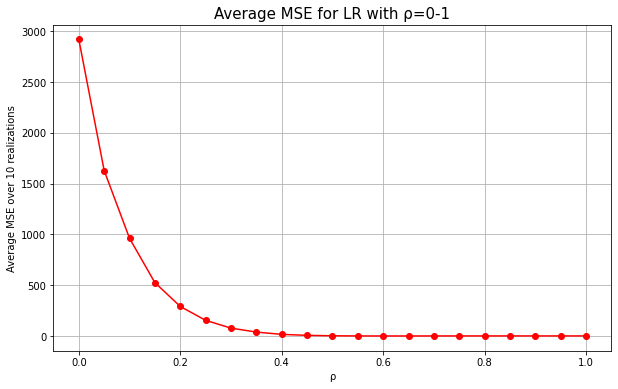
\includegraphics[width=0.6\textwidth]{../graphs/bigplot1}
    \caption{Caption for Big Plot.}
    \label{fig:bigplot1}
\end{center}
\end{figure}

Quisque ornare metus sit amet turpis accumsan aliquam. Duis condimentum sollicitudin ornare. Integer eu sodales orci. Quisque quis purus et ligula pretium posuere id eu eros, as seen in Figure~\ref{fig:bigplot1}.

\subsection{Inserting Two Figures Side-By-Side}

\begin{figure}[h]%
    \centering

    \begin{minipage}{0.45\textwidth}
        \centering
        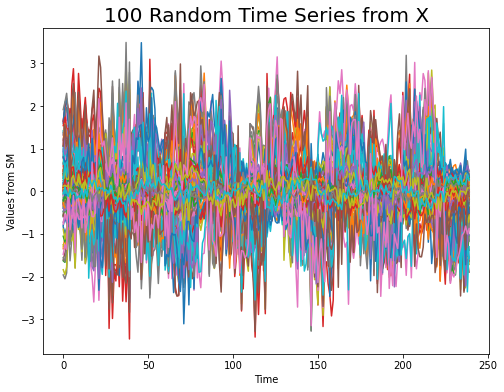
\includegraphics[width=\linewidth]{../graphs/subplot1}
        \caption{Caption for subplot1.}
        \label{fig:subplot1}
        \end{minipage}
    \hfill
    \begin{minipage}{0.45\textwidth}
        \centering
    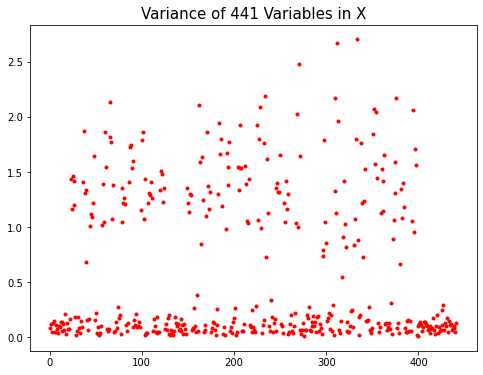
\includegraphics[width=\linewidth]{../graphs/subplot2}
    \caption{Caption for subplot2.}
    \label{fig:subplot2}
    \end{minipage}

\end{figure}

Data A can be seen in Figure~\ref{fig:subplot1}, and Data B in Figure~\ref{fig:subplot1}

\subsection{Four figures, 2 rows, 2 column}

\begin{figure}[H]% %choice: t,b,p,H
    \centering

        \begin{minipage}{0.45\textwidth}
            \centering
          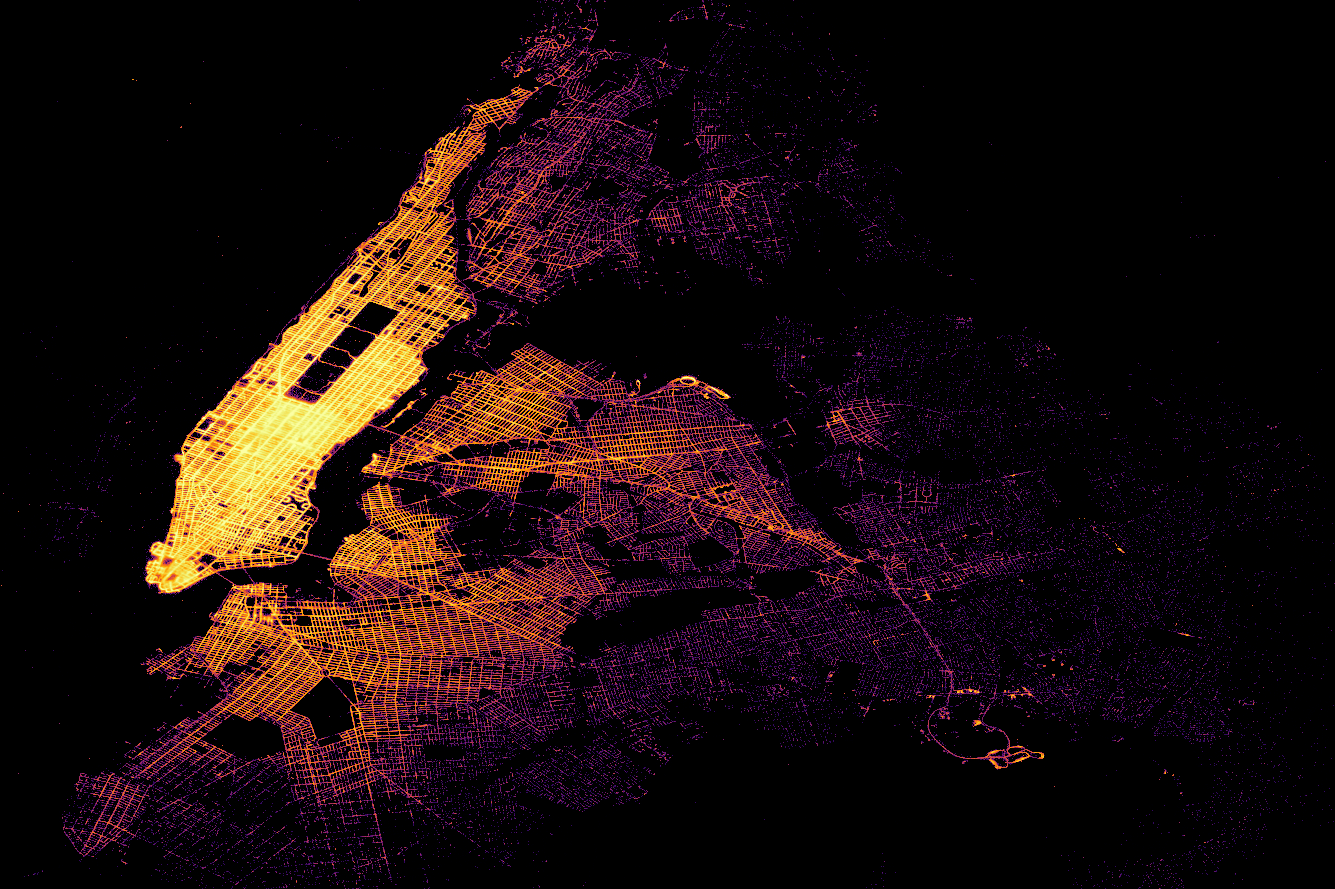
\includegraphics[width=\linewidth]{../graphs/subplot11}
          \caption{Caption for subplot 1-1.}
          \label{fig:subplot11}
        \end{minipage}
        \hfill
        \begin{minipage}{0.45\textwidth}
            \centering
          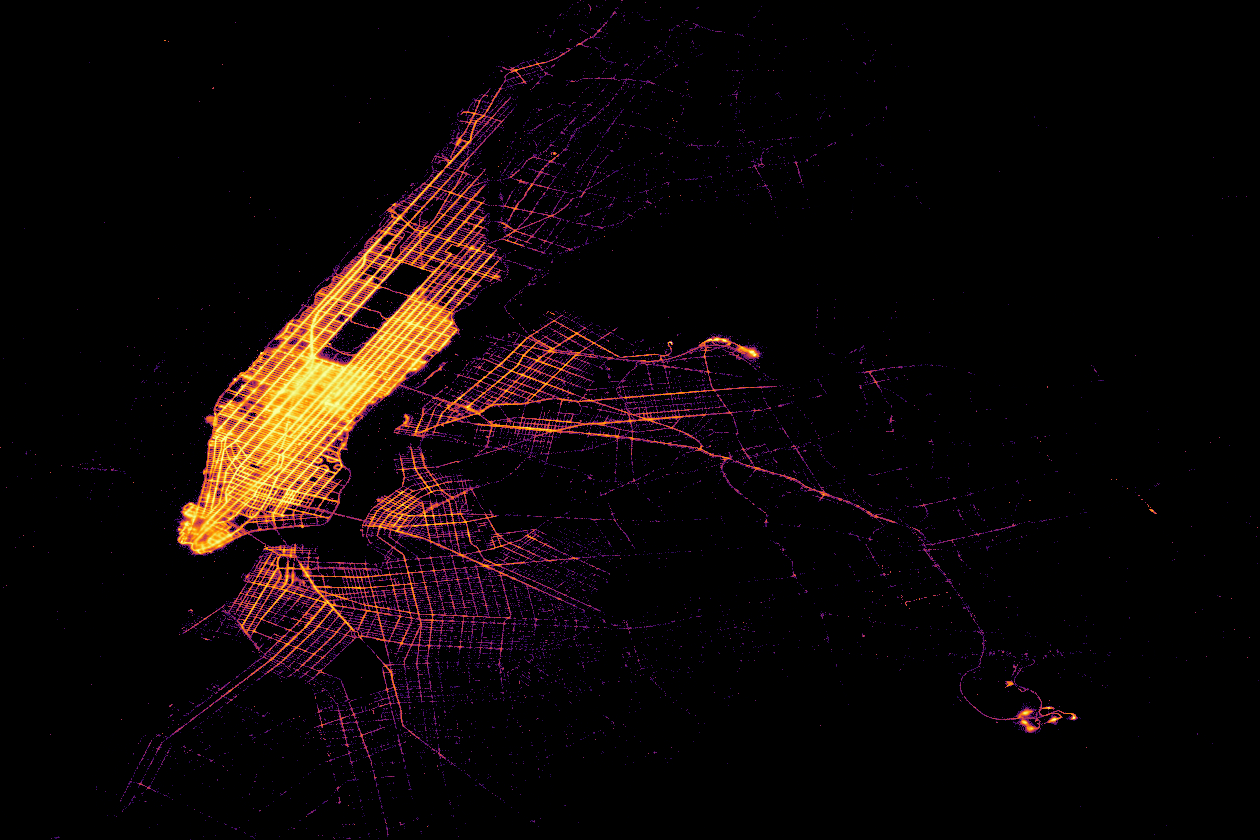
\includegraphics[width=\linewidth]{../graphs/subplot12}
          \caption{Caption for subplot 1-2.}
        \label{fig:subplot12}
        \end{minipage}

        \medskip

        \begin{minipage}{0.45\textwidth}
            \centering
            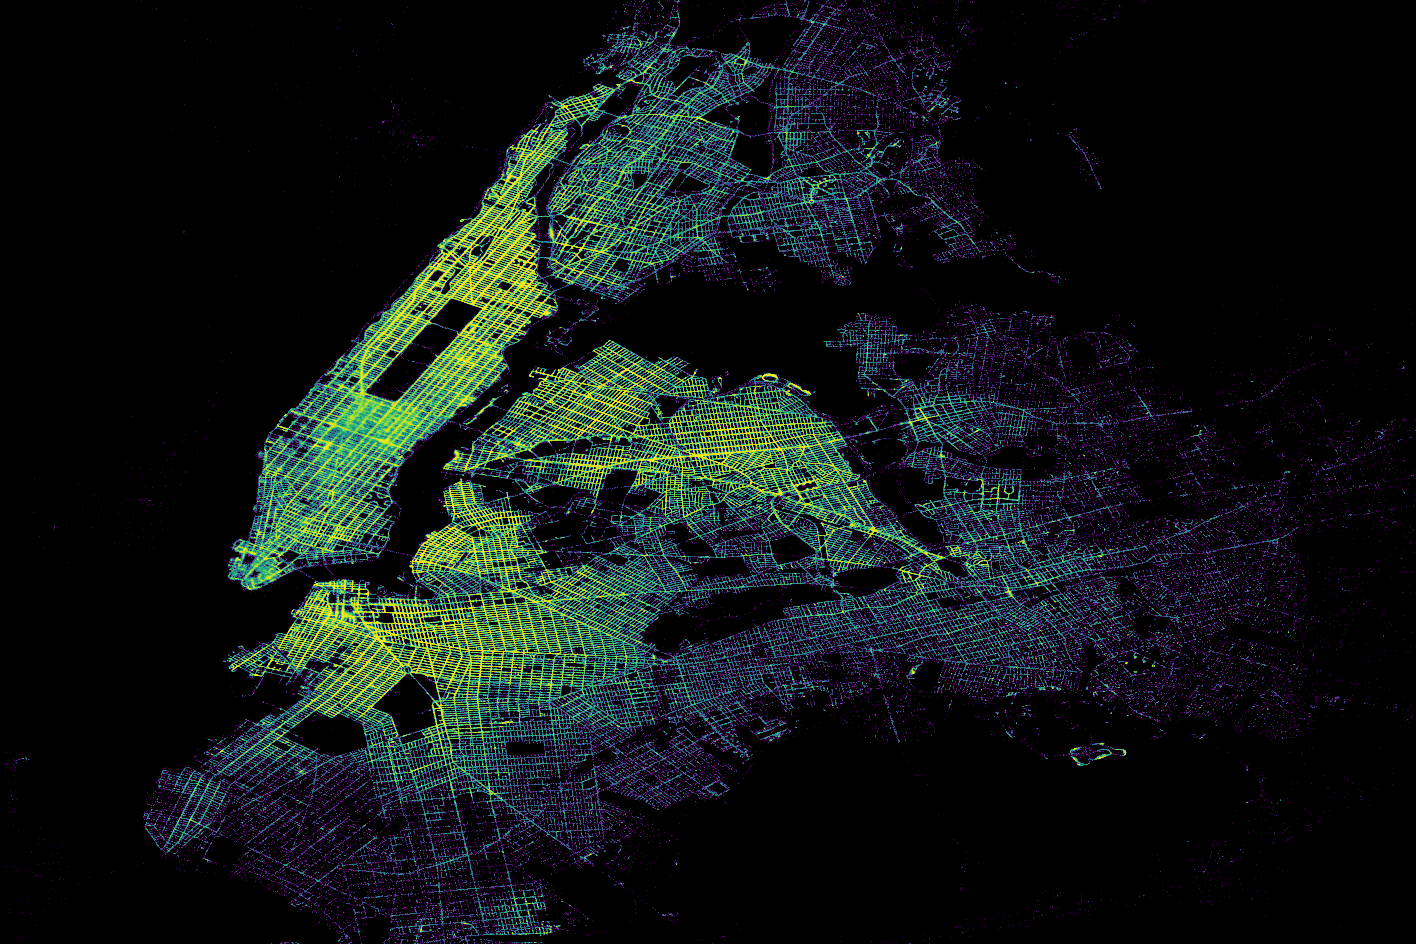
\includegraphics[width=\linewidth]{../graphs/subplot21}
            \caption{Caption for subplot 2-1.}
          \label{fig:subplot21}
          \end{minipage}
        \hfill
        \begin{minipage}{0.45\textwidth}
            \centering
        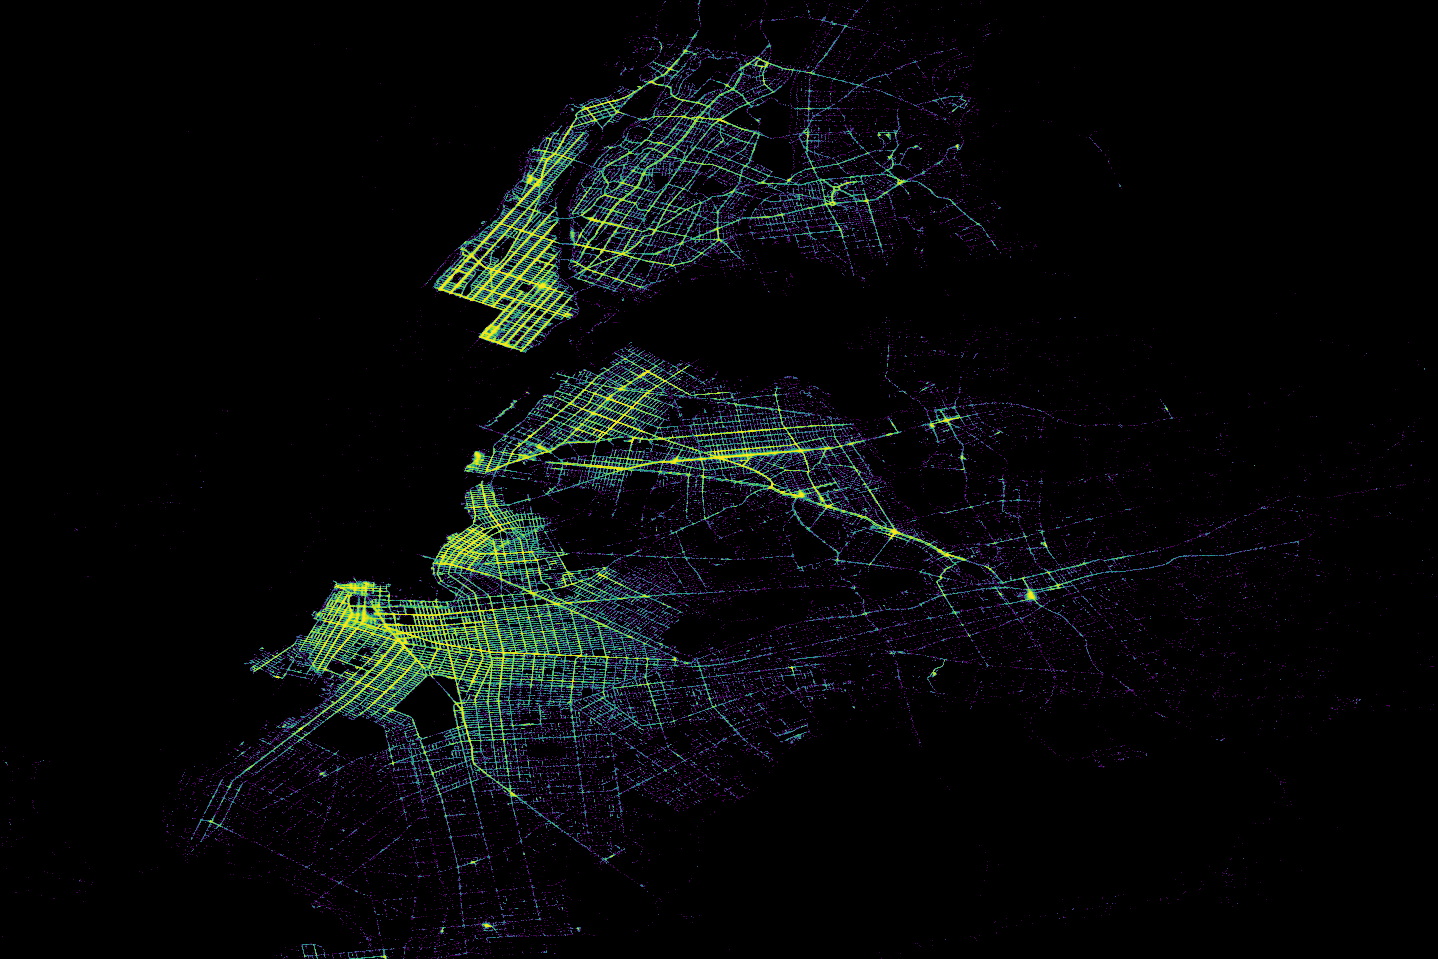
\includegraphics[width=\linewidth]{../graphs/subplot22}
        \caption{Caption for subplot 2-2.}
        \label{fig:subplot22}
        \end{minipage}

\caption{Caption for all four figures.}
\label{fig:all4plots}
\end{figure}


\subsection{Inserting Table Example}

\begin{table}[H]

    \begin{tabular}{lrrlrrrrrr}
        \toprule
            pickup\_datetime &  tempm &  tempi &      conds &  hum &  vism &  wspdm &  precipm &  rain &  fog \\
        \midrule
        2015-12-31 00:15:00 &    7.8 &   46.0 & Light Rain & 89.0 &   4.0 &    7.4 & 0.500000 &     1 &    0 \\
        2015-12-31 00:42:00 &    7.8 &   46.0 &   Overcast & 89.0 &   6.4 &    7.4 & 0.800000 &     0 &    0 \\
        2015-12-31 00:51:00 &    7.8 &   46.0 &   Overcast & 89.0 &   8.0 &    5.6 & 0.800000 &     0 &    0 \\
        2015-12-31 01:51:00 &    7.2 &   45.0 &   Overcast & 90.0 &  12.9 &    7.4 & 0.300000 &     0 &    0 \\
        2015-12-31 02:51:00 &    7.2 &   45.0 &   Overcast & 90.0 &  12.9 &    0.0 & 0.295455 &     0 &    0 \\
        \bottomrule
        
        \end{tabular}

        \caption{Caption of table.}
        \label{tab:table-name}

    \end{table}


\section{Math Equations}

This is an example of a newline equation. The Ordinary Least Squares (OLS) for this problem can be expressed as:

$$y(\mathbf{x}, \mathbf{w}) = w_0 + \sum_{j = 1}^{m} w_j x_j = \mathbf{w} \cdot \mathbf{x} $$

\begin{enumerate} 
    \item $y$ is the trip demand, the target variable to be predicted;
    \item $\mathbf{x} = [x_0, x_1, \ldots, x_m]$ is a vector of trips and weather features (where $x_0 = 1$ which is the bias); and
    \item $\mathbf{w} = [w_0, \ldots, w_m]$ are the weights for every feature.
\end{enumerate}

This is an example of an in-line equation. The Ridge Regression (RR) parameters are estimated by:

\begin{enumerate}
    \item $ \*A_{RR} = (\*D^\top \*D + \tilde{\lambda} \*I )^{-1} \*D^\top \*X $, where $ \*D = \*{TC}$ and $\tilde{\lambda} = \lambda V$.
    \item $ \*D_{RR} = \*X \*A^\top_{RR}$.
    
\end{enumerate}

\section{Methodology}
\label{section:methodology}

Ut cursus magna vel neque egestas, nec lobortis nibh lacinia. In congue diam quis justo sagittis, sit amet mattis ipsum pharetra. Vestibulum elementum dignissim urna, eget laoreet ante gravida gravida. Praesent feugiat finibus est, eget mattis nisl vulputate id. Vivamus felis sem, vulputate eget lacus eget, luctus vehicula sem. Suspendisse potenti. Morbi tincidunt interdum justo convallis condimentum. Proin quis ante ac neque sagittis euismod dignissim ut neque. Suspendisse non aliquam ligula. Nullam auctor orci nec tincidunt sodales. Nulla nec viverra purus. Vestibulum vel dignissim ante, et condimentum enim. Aenean et elementum elit, ac consectetur nisi. Pellentesque nec nibh sit amet nunc pharetra semper vel in ex.

Sed congue orci vel dolor blandit consequat. Phasellus non urna vel tellus rhoncus volutpat a et dui. Pellentesque at massa nunc. Aliquam tincidunt dapibus finibus. Pellentesque sed ante fringilla, hendrerit orci vitae, congue magna. Suspendisse tellus purus, condimentum vel venenatis ac, efficitur in sapien. Nunc interdum, purus nec tincidunt rhoncus, ante ante feugiat leo, consequat tempor nisl enim non ipsum. Donec luctus tristique lectus. Phasellus a bibendum ipsum. Fusce malesuada orci metus, eget mattis libero tincidunt quis. Aliquam in blandit felis. Curabitur ornare turpis sit amet est faucibus egestas.

\section{Results and Discussion}
\label{section:methodology}

Sed congue orci vel dolor blandit consequat. Phasellus non urna vel tellus rhoncus volutpat a et dui. Pellentesque at massa nunc. Aliquam tincidunt dapibus finibus.

\section{Conclusions}
\label{section:conclusions}

Sed erat dolor, commodo eu est non, dictum lacinia nulla. Suspendisse tempus a magna eget cursus. Sed congue leo vel lorem volutpat mattis. Integer quis tincidunt ex, rutrum posuere metus.



\clearpage

% BEGIN REFERENCES SECTION
% You may change this to use bibtex, but this is also fine if you are unsure how to do it.

\nocite{*}

\raggedright \bibliographystyle{chicago}%
\bibliography{report}%

\end{document}